\chapter{Comment être performant en athlétisme ?}
\label{part:performance}

Avant de me demander si la technologie peut permettre de mieux comprendre la performance, je vais commencer par définir la performance sportive ainsi ses déterminants.

    \section {Qu'est ce que la performance sportive ?}

        \subsection{Définition de la performance}
        
            Selon Vladimir Platonov, scientifique dans le domaine des sciences du sport, "la performance sportive exprime les possibilités maximales d'un individu dans une discipline à un moment donné de son développement". \\
            
            Pour Trilles, c'est "l'aboutissement, le point final (ou intermédiaire) d'une série d'actions appelées préparation sportive. Elle constitue l'objectif d'un long processus d'entraînement."\\
        
            Nous pouvons également dire que la performance sportive est le résultat d’adaptations motrices aux contraintes et possibilités d'une discipline. 
            Ces contraintes peuvent être d'ordre :
            \begin{itemize}
                \item Réglementaires : par exemple au 400m en athlétisme il est interdit de marcher sur la ligne intérieure de son couloir,
                \item Événementielles : adaptabilité aux évènements (comme la météo par exemple),
                \item Temporelles : par exemple en athlétisme, le temps de réaction au moment du coup de feu,
                \item Humaines : ces contraintes peuvent être dépendantes (état de forme du jour) ou indépendantes (chance) de l'athlète.\\
            \end{itemize}
        
            La résolution des problèmes posés par ces contraintes conduit l'athlète à mobiliser des ressources de différentes natures comme ses capacités motrices, techniques, physiques et mentales. Ces ressources peuvent être entretenues et développées grâce à l’entraînement.\\
            
            La performance sportive est donc à la fois \textbf{multifactorielle} car elle dépend de l'optimisation de chacun des paramètres qui concourent au résultat final et \textbf{systématique} car les différents facteurs sont interdépendants et unis par des interactions réciproques. Agir sur l'un d'entre eux n'est pas sans conséquence pour les autres.
            
        
        \subsection{Éléments constitutifs de la performance}
        
            La performance sportive est constituée de deux parties : visible et invisible.\\
            
            La partie visible est celle dont nous faisons référence communément lorsque nous évoquons la performance. C'est un résultat qui peut être définit par un temps à l'arrivée d'une course, une distance parcourue ou bien un classement. C'est donc un élément quantifiable.\\
            
            La partie invisible pourrait quant à elle être définit comme tout ce qui se produit dans notre corps et plus précisément au niveau physiologique lors d'une course. Ce coté de la performance n'est généralement pas analysé par les entraîneurs et athlètes car elle demande des outils spécifiques et une réelle étude pour trouver des résultats exploitables et intéressants. C'est sur cette partie que portera mon mémoire. 
    
        \vspace{10pt}
    
    \section {Les facteurs de la performance en athlétisme}
    
        La performance sportive est un phénomène complexe qui s’articule autour d'un mélange de différents facteurs qui peuvent être indépendants de l'athlète (environnement, chance etc), innés (morphologie, patrimoine génétique) ou encore acquis grâce à l'entraînement (physique, mental etc).\\
        
        Dans les disciplines de courses en athlétisme, on peut séparer les paramètres qui influencent la performance en 6 catégories qui ont eux mêmes des sous-catégories : 
        \begin{itemize}
            \item Neuromusculaires et relatifs à la condition physique
            \item Psychologiques
            \item Environnement social
            \item Chance
            \item Entraînement invisible
            \item Facteurs physiologiques
        \end{itemize}

        \begin{figure}[H]
            \centering
            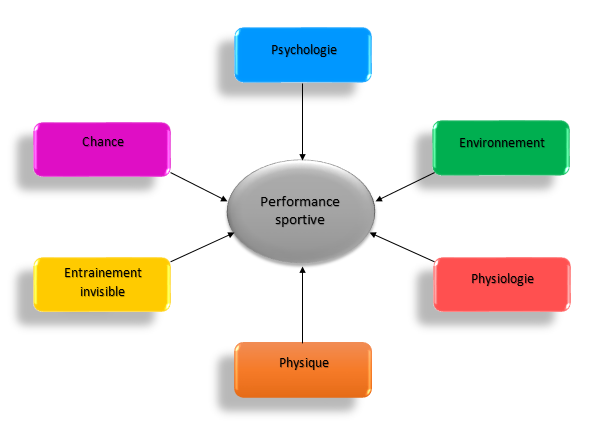
\includegraphics[scale=0.7]{images/facteursPerf}
            \caption{\label{fig:filieres-energetiques}Facteurs de la performance en athlétisme}
        \end{figure}
        
        \subsection{Facteurs neuromusculaires et relatifs à la condition physique}
        
        Les facteurs neuromusculaires concernent la relation entre le système nerveux et le système musculo-squelettique. Ils permettent donc aux muscles de se contracter en fonction des différentes informations reçues.\\
        
        Ces facteurs sont généralement les plus complets et représentent les aspects de la performance qui occupent le plus grand degré de concentration et de temps de préparation. En effet, dans de nombreux sports, peu importe la façon dont l'athlète se consacre à l'entraînement, s'il n'est pas physiquement équipé pour concourir, la performance ne s'améliorera pas.\\
        
        La composante neuromusculaire de la performance sportive est subdivisée en ses propres éléments discrets qui doivent chacun faire l'objet d'entraînements spécifiques.
        
        Les différents types d'entraînements concernent :
            \begin{itemize}
                \item Les filières énergétiques
                \item La force musculaire
                \item La souplesse
                \item La technique de course\\
            \end{itemize}
        
        Ces entraînements sont influencés par l'anatomie de l'athlète et la distribution de ses fibres. En effet, les muscles sont composés essentiellement de fibres musculaires.\\
      
        On compte deux grands types de fibres musculaires :
        \begin{itemize}
            \item \textbf{Les fibres rouges} (fibres lentes de type I) : peu de vitesse et peu de force mais grande forte capacité de résistance à l’effort (endurance),
            \item \textbf{Les fibres blanches} (fibres rapides de type II) : vitesse de contraction rapide et beaucoup de force mais faible résistance à l’effort et incapables de se contracter longtemps (peu d'endurance).\\
        \end{itemize}
        
        \begin{figure}[H]
            \centering
            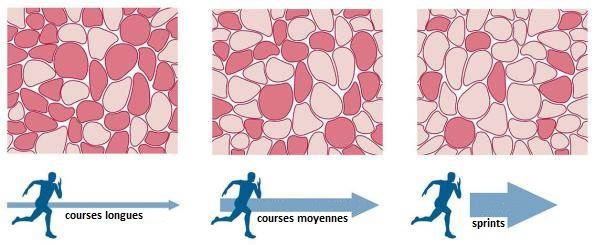
\includegraphics[scale=0.7]{images/fibres.jpg}
            \caption{\label{fig:filieres-energetiques}Fibres sollicitées lors de différents types de courses}
        \end{figure}
        
        A la naissance, la répartition des fibres, et donc la composition des muscles, est programmée génétiquement pour 50\%. Cela signifie que la moitié de nos fibres musculaires sera non modifiable et l’autre moitié sera transformable par l’entraînement.\\
        
        De plus, pour se contracter le muscle a besoin d'un apport en énergie, et cette dernière doit être disponible au cœur même de la fibre musculaire.\\
        
        C'est donc en fonction des prédispositions génétiques de l'athlète, de ses aptitudes physiologiques et musculaires ainsi que de sa discipline que l'athlète va produire l'énergie nécessaire à l'accomplissement de son effort.\\
      
        Il existe trois modes de production d'énergie : 
        \begin{enumerate}
            \item La filière anaérobie alactique (sans oxygène et sans production de lactates) 
            \item La filière anaérobie lactique (sans oxygène et avec production de lactates)
            \item La filière aérobie (avec oxygène)\\
        \end{enumerate}
        
        Chaque d’elle est caractérisée par une capacité (quantité totale d'énergie potentielle) et une puissance (quantité d'énergie délivrable par unité de temps). Par comparaison avec un réservoir muni d'un robinet, la capacité correspond au volume du réservoir et la puissance au débit du robinet. 
        Bien que fonctionnant en parallèle, ces filières possèdent des durées de fonctionnement spécifiques qui les prédisposent à trois types d'efforts différents.
        
        \paragraph{La filière anaérobie alactique}
        correspond à la vitesse et est construite par une formation axée sur le développement des fibres à contraction rapide des muscles. 
        Cette filière s’enclenche dès les premières secondes de l’exercice et est utilisée essentiellement dans les efforts réalisés au maximum d’intensité en un temps inférieur à 20 secondes. Cependant, sollicitée à son maximum d’intensité, la filière anaérobie alactique est épuisée au bout de 7 secondes. En athlétisme les disciplines concernées par ce métabolisme énergétique sont les sprints explosifs tels que le 100 mètres.  Pour les courses plus longues (200 m, 400 m, 800 m), et les courses de haies (110 m haies et 400 m haies), le métabolisme anaérobie alactique est mis en jeu lors des 7 à 20 premières secondes. Ensuite c'est la filière anaérobie lactique qui prend le relais.
        
        
        \paragraph{La filière anaérobie lactique}
        se met en place lorsqu'il n’y a plus assez d’arrivée d’oxygène pour répondre à l’effort supérieur. Le corps fait alors appel à cette filière, qui consiste en une aide au fonctionnement du muscle. Cependant cette aide n’est pas sans conséquences car la filière anaérobie lactique utilise du glycogène, un sucre complexe présent à l'état de réserve au niveau du muscle, qui à la suite de réactions chimiques complexes, se transforme en lactate. L'accumulation de lactates dans le sang entraîne un apport d’acidité dans l’organisme qui perturbe la contraction du muscle.
        Résultat, la fatigue musculaire se fait sentir et la faculté de poursuivre son effort se réduit. 
        
        Ce métabolisme s’enclenche dès les premières secondes de l’exercice mais avec une intensité inférieure à celle du processus anaérobie alactique.
        Il assure des efforts de puissance élevée et de durée moyenne, de 20 à 45 secondes. 
        
        C'est ce processus qui prédomine dans les courses de résistance comme le 400m. 
        
        
        \paragraph{La filière aérobie}
        représente les gammes d’intensité de travail d’endurance et est mis en place lors d'un effort long et modéré.
        Elle s'enclenche également dés le début de l'effort mais c'est au bout de 3 min qu'elle devient la seule source d'énergie étant donnée que les deux autres ont été épuisées.
        La filière aérobie correspond à l’aptitude de l’organisme à capturer (respiration), transporter (globules rouges + débit cardiaque) et utiliser (efficacité oxydative des cellules) l’oxygène pour transformer l’énergie.
         
        C'est une qualité essentielle au succès quelle que soit la spécialité car elle permet de régénérer les sources précédentes\\
         
        Contrairement à ce que l'on pourrait penser, même dans les disciplines de courte durée et à haute intensité telles que le sprint par exemple, l'aérobie tient un rôle très important car elle permet une meilleure oxygénation des muscles et participe à l’élimination des déchets de la contraction musculaire ce qui favorise une récupération plus rapide et plus efficace après un entraînement ou une compétition. \\
        
        Dans les disciplines de fond, l'aérobie est un aspect central car la capacité de l'athlète à consommer et traiter l'oxygène est primordiale. En effet, un des axes de travail du processus aérobie est de maintenir une intensité élevée le plus longtemps possible tout en dépensant le moins d'énergie possible.
        
        Cependant ce processus n'est pas sans limite. 
        Lorsque l’athlète se rapproche du seuil critique du processus aérobie c'est à dire des limites pour lesquelles tout l’oxygène disponible au niveau musculaire est utilisé, on dit qu'il atteint sa puissance maximale aérobie (PMA) ou VO2Max (débit maximum d’oxygène). 
        
        Néanmoins, un athlète ayant atteint sa PMA peut encore augmenter l’intensité de son exercice. Ne disposant plus de réserves d’oxygène, il fera à nouveau appel à ses processus anaérobies, ce qui va provoquer une augmentation importante de la lactatémie. C’est le cas par exemple lors du sprint final d’un 1500m.
        
        
        \begin{figure}[H]
        \centering
        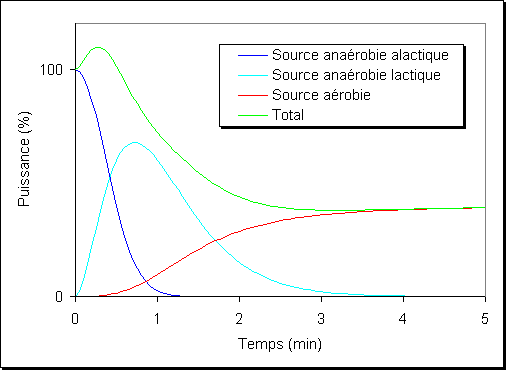
\includegraphics[scale=0.7]{images/aerobie-anaerobie-alactique2.png}
        \caption{\label{fig:filieres-energetiques}Les filières énergétiques}
         \end{figure}
         
         Dans le schéma suivant, on peut clairement voir que les trois sources ne sont pas indépendantes. Elles fonctionnent en parallèle, à des degrés divers, ce qui crée une illusion de fonctionnement en série. Pour chaque source, la surface comprise entre la courbe et l'axe du temps représente la capacité (l'endurance).\\
         
         La filière anaérobie alactique est celle qui produit le plus de puissance mais qui a la plus faible capacité c'est à dire qu'elle ne fournit pas d'énergie aux muscles longtemps : elle ne peut pas prolonger un effort à 100\% de sa VMA plus de 7 secondes. Au-delà de cette période, les muscles doivent utiliser d’autres procédés pour continuer la couverture énergétique. C'est le métabolisme anaérobie lactique qui prend le relais. Cette filière a une capacité et une puissance moyenne. Elle est active jusqu'à 3 min d'effort mais produit une puissance élevée jusqu'à 45 secondes d'effort. Ensuite, la réserve d'énergie s'affaiblie et c'est la filière aérobie qui prend le relais. Ce métabolisme a une endurance très supérieure à celles des processus anaérobies mais une puissance inférieure à celle assurée par ces derniers. A partir d'environ 3 minutes d'effort elle devient la seule source d'énergie et elle délivre sa puissance maximale vers 3 minutes 30 d'effort.
         
         
         \vspace{10pt}
        
        La distribution des fibres à travers les muscles est donc régulée par la génétique, mais cette distribution n'est pas irréversible.  
        Le but de l'entraînement est d'entraîner les fibres pour maximiser leurs effets afin d'être le plus efficace possible mais également d'augmenter les capacités et la puissance(faculté à produire une grande énergie dans un temps le plus court possible) de l'athlète dans les filières énergétiques les plus importantes selon sa spécialité. 
        
        
        En plus des entraînements pour augmenter ses capacités énergétiques, l'athlète travaille aussi sa souplesse.
                
            
        \subsubsection{La souplesse}
        La souplesse désigne la qualité physique permettant d’accomplir des mouvements corporels avec la plus grande amplitude (articulaire et musculaire) et aisance possibles. que ce soit d’une manière active (en mouvement dynamique) ou passive (sans mouvement dynamique).
    
         On peut distinguer différents types de souplesse :
         \begin{itemize}
             \item la souplesse générale : mobilise les systèmes musculaires et articulaires pour faire en sorte d’apporter une aisance gestuelle.
             \item la souplesse spécifique : se rapporte à un muscle ou une articulation spécifique (Franchir des haies nécessite une grande souplesse au niveau des ischios jambiers).
             \item la souplesse statique et dynamique : résulte de la présence ou non d’un mouvement.
             \item la souplesse active et passive : concerne la souplesse statique, leur différence réside dans la présence ou non d’une contraction musculaire.\\
         \end{itemize}

        En athlétisme, la souplesse est une qualité essentielle : 
        plus l'amplitude de mouvement présente dans les articulations d'un athlète est grande, plus l’efficacité du geste et la capacité de mouvement dynamique est grande.\\

        La souplesse se travaille grâce à des étirements.\\
        
        Il existe deux types d'étirements: 
        \begin{itemize}
            \item Les étirements avant séance :  pour réveiller les muscles mais aussi augmenter et faciliter les amplitudes articulaires et musculaires (allongement des tissus et des muscles) qui seront utilisés lors de l'effort.
            \item Les étirements après séance : pour permettre aux muscles de récupérer mais aussi de prévenir les blessures.
            Il s’agit donc de relâcher et de décontracter les muscles pour retrouver un degré de tonus musculaire presque similaire au début de l’effort.
        \end{itemize}
                
            
        \vspace{10pt}
            
            
        \subsubsection{La technique}
        
        En athlétisme, la maîtrise technique est un aspect indispensable pour le haut niveau.
        
        Cela englobe :
        \begin{itemize}
            \item la qualité des gestes (placements du corps et des articulations)
            \item la précision technique (pose de pied sous le bassin par exemple)
            \item la vitesse d’exécution (qui dépend aussi de la qualité et précision des gestes)
            \item la capacité de coordination
        \end{itemize}
        
        Généralement la technique n'est pas innée et se travaille grâce à la répétition et à des exercices spécifiques.
        
        Il n'y a pas une seule technique efficace et universelle mais plutôt une technique adaptée à chaque athlète en fonction du type de corps et des capacités musculaires de chacun.
        
    
        Ces différents facteurs ne sont pas les seuls déterminants de la performance en athlétisme. Je vais maintenant m'intéresser à d'autres facteurs tout aussi importants.\\
        
        \vspace{10pt}
            
                
        \subsection{Facteur psychologique}

            Le contrôle mental et les aspects psychologiques associés à la performance sportive sont des éléments déterminants qui se reflètent dans le résultat final de l'effort de l'athlète.\\
            
            En athlétisme, on dit que le mental joue pour 70\% de la performance et le physique pour seulement 30\%. C'est entre autres lui qui sépare les athlètes qui réussissent de ceux simplement talentueux.
            
            Cependant, les éléments mentaux du sport sont à bien des égards les plus difficiles à maîtriser, car ils requièrent habituellement un haut niveau de maturité et d'expérience athlétique pour aboutir à des résultats.\\
            
            Il n'est en effet pas rare de trouver des athlètes extrêmement doué physiquement mais qui sont incapable de gérer la pression et de maîtriser leurs émotions pendant une compétition. Nous pouvons prendre l'exemple de Marie-José Perec, athlète surdouée et multiple médaillée olympique dans les épreuves de 200 et 400m mais qui avait précipitamment quitté les Jeux Olympiques la veille de sa course sans explications.\\
            
            Les capacités cognitives de l'athlète peuvent expliquer certains comportements car elles sont directement impliquées dans le processus mental. En effet, celles ci concourent à l’appréhension et au traitement des informations ainsi qu'à l’analyse des situations. Elles se manifestent par un certain nombre de processus mentaux comme l’intelligence, la mémoire, le langage etc. Le fait d'avoir une grande puissance analytique permet à athlète de prendre le contrôle de ses émotions et ainsi rester calme en situation de stress ou sous pression.
         
            Cependant la maîtrise émotionnelle n'est pas le seul point important de la force mental d'un athlète.\\
            
            La capacité du sportif à avoir confiance en soi ainsi que son aptitude à être persévérant pour poursuivre son objectif jusqu’au bout quelles que soient les difficultés rencontrées sont également des qualités primordiales.\\
            
            Enfin, une des clés essentielles du succès est d'avoir un désir de réussite hors du commun. C'est cette envie qui permettra à l'athlète d'accepter la souffrance tout en se faisant plaisir, de s'auto-motiver et de pouvoir se surpasser tant en compétition qu'à l'entraînement.\\
            
                
        \vspace{10pt}
                
                
        \subsection{Facteur social}
            
            L'athlète est un compétiteur mais aussi et avant tout un être humain évoluant dans un environnement et un contexte social au quotidien.\\
            
            Nous pouvons définir l’environnement comme étant un ensemble de conditions et de processus, englobant le système "entraînement-compétition" et plus globalement, la vie de l'athlète. \\
            
            Cet environnement peut être : 
            \begin{itemize}[label=\textbullet, font=\LARGE \color{blue}]
                \item Matériel : piste par exemple,
                \item Physique : conditions climatiques, altitude
                \item Sportif : logique de formation / compétition, catégories et niveaux des athlètes,
                \item Fédéral : calendrier des compétitions
                \item Relationnel : dynamique au sein du groupe d’entraînement, situation familiale, affective ou professionnelle, relation entraîneur/entraîné \\
            \end{itemize}

            Les pensées, sentiments et comportements de l'athlète sont influencés par son environnement et notamment par la présence réelle, imaginaire ou implicite des personnes qui gravitent autour de lui. La relation entraîneur/entraîné est un des éléments, si ce n'est l'élément le plus important dans l'environnement d'un sportif. Elle est généralement basée sur une entente entre une personne qui veut atteindre des objectifs et un guide qui peut l’y amener. Ce lien repose donc sur un désir de performance et peut être de différentes natures : amical, mentor/athlète, fraternel etc. Quelle que soit la nature de cette relation, l'athlète et l'entraîneur passent environ 4h à 5h par jour ensemble dans le but d'atteindre un objectif commun. La qualité de la communication et la confiance entre les deux individus sont donc des éléments indispensables et déterminants dans leur quête de la réussite.\\
            
            Dans cette relation, le rôle de l'entraîneur est primordial. C'est lui qui va organiser les entraînements afin de favoriser le développement des capacités de l'athlète et l'amener à l'accomplissement de ses objectifs. C'est donc un gestionnaire mais pas que. En effet, c'est également la personne qui va lui inspirer confiance et le soutenir dans les moments de doutes, qui va l'aider à utiliser des ressources connues ou inconnues pour solutionner un problème mais également celui qui va aider l'athlète dans son développement personnel afin d'augmenter son bien-être au quotidien.\\
         
         
            L'environnement social de l'athlète module et influence l'organisation et la gestion des entraînements/compétitions mais aussi leur réalisation.
            Cependant les facteurs environnementaux sont rarement sous le contrôle personnel de l'athlète. La capacité de l'athlète à s'adapter à des facteurs environnementaux différents et inattendus est souvent déterminante pour la réussite. \\
            
                
        \vspace{10pt}
            
            
        \subsection{Facteur chance}    
            
            Le facteur chance est un facteur qui peut être controversé mais qui existe néanmoins. Il conditionne les éléments extérieurs et non contrôlables autour de la performance.\\
            
            Le facteur chance englobe :
            \begin{itemize}
                \item Le nombre et le niveau des adversaires
                \item Les éventuelles blessures et abandons des adversaires
                \item Les erreurs de jugement (athlète disqualifié par erreur par exemple)
                \item La configuration des séries et des couloirs. En athlétisme le couloir 1 est le plus mauvais couloir en terme de rapidité du fait de sa proximité a
                vec le centre du stade. Cependant, lors des séries, les couloirs sont tirés au  hasard donc il est possible de l'avoir. Un autre exemple ou la chance entre en jeu est lors de la configuration des couloirs par rapport aux concurrents : un athlète qui est au couloir 5 aura un avantage par rapport à celui qui est au couloir 6 car il bénéficiera du visuel sur lui. Il pourra donc le contrôler plus facilement et éviter des surprises.
                \item Les conditions météorologiques. Ces conditions sont un facteur qui sera le même pour tous les concurrents. Il faudra donc avoir une meilleure capacité d'adaptation que les autres.
            \end{itemize}
            
            Pour un athlète cherchant à maximiser sa performance, il ne doit pas seulement exercer un contrôle mental pour éviter d'être dérangé par ces conditions mais il doit également examiner les moyens de faire fonctionner les conditions dans le positif.
            
            
        \vspace{10pt}
             
             
        \subsection{L'entraînement invisible}
         
            Chaque séance d’entraînement, chaque compétition provoque une dépense énergétique proportionnelle à l’intensité et la durée de la sollicitation musculaire. 
             
            L'entraînement invisible correspond à optimiser tout ce qui tourne autour de l'entraînement physique pour rentabiliser au maximum ses effets. Il s’agit des domaines que l’on pourrait classer dans l’hygiène de vie et qui permettent d'optimiser la récupération. \\
            
            Concrètement, cela consiste à se préparer au mieux à l’effort, à optimiser son alimentation pour restaurer les réserves énergétiques et les tissus utilisés ainsi qu'à s'entretenir par des soins divers, tout cela pour éviter le surentraînement et prévenir l'apparition de blessures.\\
            
            Le surentraînement est un phénomène qui intervient lorsque la durée la durée de récupération entre les séances n’est pas respectée ou mal gérée. Cela engendre une accumulation de la fatigue et une régression progressive des capacités physiques de l'athlète. Il est donc primordial de trouver le  bon équilibre entre activité physique (entraînement, compétition) et récupération (repos, alimentation, soins..). Cette phase de récupération va permettre à l'ensemble des systèmes sollicités pendant l’effort de se restructurer et la régénération des réserves énergétiques.\\
              
            La récupération est donc l'une des clés de la performance.\\
    
            Les paramètres d'une bonne récupération sont : 
             \begin{itemize}
                 \item Le sommeil
                 \item L'alimentation et l'hydratation
                 \item Le suivi médical
             \end{itemize}
             
            Beaucoup d'athlètes néglige partiellement ou totalement l'entraînement invisible pourtant il est tout aussi important que l'entraînement physique. \\
            
    
                \subsubsection{Le sommeil}
        
                    Il est reconnu qu’un manque de sommeil ou un sommeil perturbé peut nuire au fonctionnement mental et physique, affaiblir le système immunitaire et affecter les autres processus de rétablissement importants pour les athlètes.
                    
                    Un sommeil de qualité est donc indispensable pour un athlète. En effet, c’est pendant le sommeil qu’il y a une grande circulation des hormones de croissance et donc une régénération des tissus cellulaires endommagés par l’entraînement. Il permet ainsi à l’organisme de récupérer des efforts qu’il a fournis. 
                    
                    Une bonne nuit de sommeil se caractérise par :
                    \begin{itemize}
                        \item Le besoin en sommeil. La quantité de sommeil nécessaire diffère selon chacun mais un athlète ne devrait pas dormir moins de 8 heures par nuit. Elle peut être complétée si nécessaire par des siestes.
                     
                        \item La qualité du sommeil. Plusieurs athlètes dorment suffisamment d’heures,
                        mais leur sommeil est de mauvaise qualité. Le sommeil n'est alors pas aussi réparateur.
                        \item Le moment du sommeil. Chaque athlète présente un chronotype particulier (préférence de l’individu à réaliser une activité à certaines périodes de la journée plutôt qu’à d’autres) : certains sont matinaux et d'autres non. Les horaires d'entraînement doivent donc être synchronisés avec le rythme de l'athlète pour ne pas perturber son besoin en sommeil.
                        \item Les habitudes de sommeil. Il est important d'adopter des habitudes de sommeil pour favoriser la récupération. Par exemple, instaurer des heures de coucher avant minuit car celles ci sont les plus "récupératrices".
                    \end{itemize}
                
            
                \subsubsection{L'alimentation et l’hydratation}
                
                    Le corps humain a besoin d’apports externes pour faire fonctionner l’organisme et créer de l’énergie. Ces apports proviennent de l'alimentation et de l'hydratation quotidienne et sont d'autant plus importants chez un athlète du fait de ses hautes dépenses énergétiques.
                    Ils doivent comblés quantitativement et qualitativement les dépenses énergétiques de l'athlète afin de reconstituer les stocks d'énergie perdus.\\
                    
                    Outre la quantité et la qualité des apports, la répartition quotidienne des prises alimentaires doit être respectée : l’organisme doit être suffisamment alimenté avant l'effort pour pouvoir être performant, mais aussi après pour restaurer ses réserves énergétiques et se réhydrater.\\
                    
                    Après un effort intense, l'athlète dispose d'une "fenêtre métabolique" qui correspond à un intervalle de temps pendant lequel les aliments ingérés sont assimilés plus rapidement. C'est donc le moment favorable pour rétablir le stock d'énergie c'est à dire le stock de glycogène musculaire. 
                    
                    Ce phénomène prédomine durant la première heure après l’effort et diminue rapidement. Si l'apport glucidique n'est pas absorbé par l'athlète dans les 4 heures après l'effort, il lui faudra 3 jours pour récupérer à 100\%.
                    
                    \begin{figure}[H]
                        \centering
                        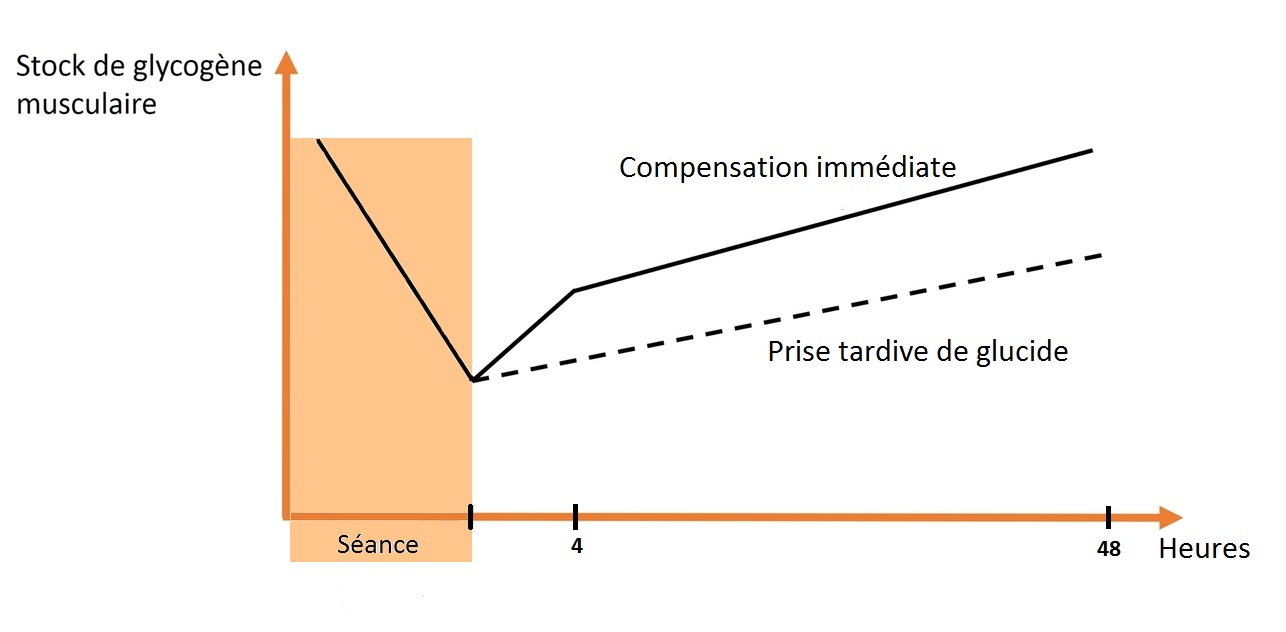
\includegraphics[scale=1]{images/fenetre-metabolique.jpg}
                        \caption{\label{fig:filieres-energetiques}La fenêtre métabolique}
                    \end{figure}
                    
                    
                    De la même façon, il est important d’assurer un bon équilibre hydrique en s'hydratant régulièrement, mais aussi d'adapter son apport en eau en fonction des pratiques en buvant avant, pendant et après l’effort. En effet, la transpiration et la sudation entraînent une perte d'eau supplémentaire. Lorsque la perte d’eau correspond à 2\% du poids de corps, la performance baisse de 20\%, si cette perte correspond à 4\% du poids de corps, à 18° de température ambiante la performance baisse de 40\%!  De plus, l'eau favorisera la restauration du stock minéral perdu et contribuera à diminuer l’acidité musculaire dû à un l'effort.
    
             
                \subsubsection{Les soins}
       
                    Pour un athlète, le corps est l'élément indispensable à la réalisation de l’objectif qu’il s’est fixé. Cependant les entraînements quotidiens malmènent les muscles, tendons, articulations etc.  Il faut donc prendre soin de son corps et faire en sorte qu'il soit dans le meilleure état possible pour affronter les lourdes charges d'entraînements. Il faut également que l'organisme consacre toute son énergie à régénérer ses réserves au lieu de lutter contre les inflammations et les blessures.\\
                    
                    Pour cela, le sportif doit réaliser des soins qui permettront de prévenir les blessures ou de les traiter mais aussi à récupérer (soins dentaires, podologie, ostéopathie, kinésithérapie, sophrologie, cryothérapie, étirements, massages etc).
        
                
        \vspace{10pt}        
                
        \subsection{Facteurs physiologiques}
        
        Les facteurs physiologiques sont les éléments qui permettre de rendre visible la partie invisible de la performance.
        Ils concernent le fonctionnement et l'organisation mécanique, physique et biochimique des organismes vivants et leurs composants (organes, tissus, cellules et organites cellulaires).
        
        La physiologie sportive est la physiologie de l'activité physique, c'est-à-dire, l'étude des réponses et des adaptations chroniques à un grand nombre de conditions d'exercice physique
        La physiologie du sport étudie plus particulièrement l’adaptation du corps à l’exercice, les aspects de la nutrition du sportif ainsi que les fonctions motrices du corps humain dites de locomotion. L’étude des systèmes nerveux, circulatoires, cardio-vasculaires et respiratoires finit de compléter les éléments de la physiologie du sport.
L’étude de la physiologie sportive permet à l’entraîneur sportif d’élaborer des programmes de préparation physique professionnels adaptés au comportement physiologique du sportif. 
    
        Qualité biologique : capacité vital, pourcentage de masse grasse, âge osseux, consommation  maximal d’O2 et répartitions des fibres.


            Facteurs sur lesquels va porter mon mémoire 
            En athlétisme :
            Lactatemie (acide lactique)
            Acidose
            Glycémie
            Poul
            Créatinine
            
            
            Dans mon mémoire je m'intéresserais à la lactatémie, la glycémie, le poul...

        \subsubsection{Glycemie}
        \label{subsection:glycemie}
        
        \subsubsection{Lactatémie}
        \label{subsection:lactatemie}
        La lactatémie est le taux de lactate dans le sang (mmol/ L). Elle se mesure par prélèvement de goutte de sang à l'oreille, ou à l'index. On extrapole ensuite le résultat à l'échelle du litre.
        
        Le lactate est produit en raison d’une demande énergétique importante au cours de l’exercice de haute intensité, et il peut servir à la fois de régulateur de pH musculaire, mais aussi de carburant pour les fibres lentes. Nous allons maintenant appréhender le lactate comme un marqueur indirect de la sollicitation du métabolisme énergétique au cours de différentes disciplines sportives.

        \vspace{10pt}
        
    \section {Comment être performant en athlétisme}

    Maximisation de tous les facteurs
    
    Tous ces facteurs sont les fondements de la performance. Ils se révèlent plus ou moins importants selon la situation, les caractéristiques de l’athlète et du contexte de la compétition.

les facteurs déterminants doivent être connus et intégrés dans le processus d’entraînement.

C’est donc un système complet et organisé qui comprend tout ce qui englobe l’entraînement du sportif et l’ensemble des conditions dans lesquelles il évolue.

En effet, il s’agit de mettre en phase le processus d’entrainement, de le rationaliser pour arriver à la performance : gestion des charges d’entrainement, organisation du processus d’entrainement, quantification des charges, connaissance des adaptations physiologiques consécutives à l’entrainement, gestion de la fatigue et du surentrainement.

Capacité à être performant le jour J
    
    

%%% Local Variables: 
%%% mode: latex
%%% TeX-master: "memoire"
%%% End:

concentration de lactate dans le sang --> lactatémie



